%% Preamble
% Document type, packages imported, theme and color:
\documentclass{beamer}
\usepackage{amsmath,geometry,graphicx}
\usetheme{Madrid}

% Title page
\title{Light reflections}

\date{July 25, 2018}
\author{
Michael Byrne, 
Fatoumata Sanogo,
Pai Song,
Kevin Tsai,
Hang Yang, and
Li Zhu\\
\medskip
Problem Presenter:  John Peach (MIT Lincoln Lab)\\
Faculty Mentor: Alen Alexanderian (NCSU)
}
\titlegraphic{
\includegraphics[width=.5\textwidth]{./figs/title-page-image.png}}
\institute[Abbreviation]{SAMSI-IMSM}

%% Presentation
\begin{document}

% Title page:
\begin{frame}
\titlepage
\end{frame}

% Presentation overview:
\begin{frame}
\frametitle{Overview}
\tableofcontents
\end{frame}


\begin{frame}
\frametitle{First slide}

\begin{frame}[t]
\frametitle{Optical cross section}
\begin{itemize}
\item Accumulated reflectance over a target surface
\item Discrete: summing triangular facets (5 -- 20,000+) 
\item Continuous: chebfun in conjunction with R-functions
\end{itemize}
\centerline{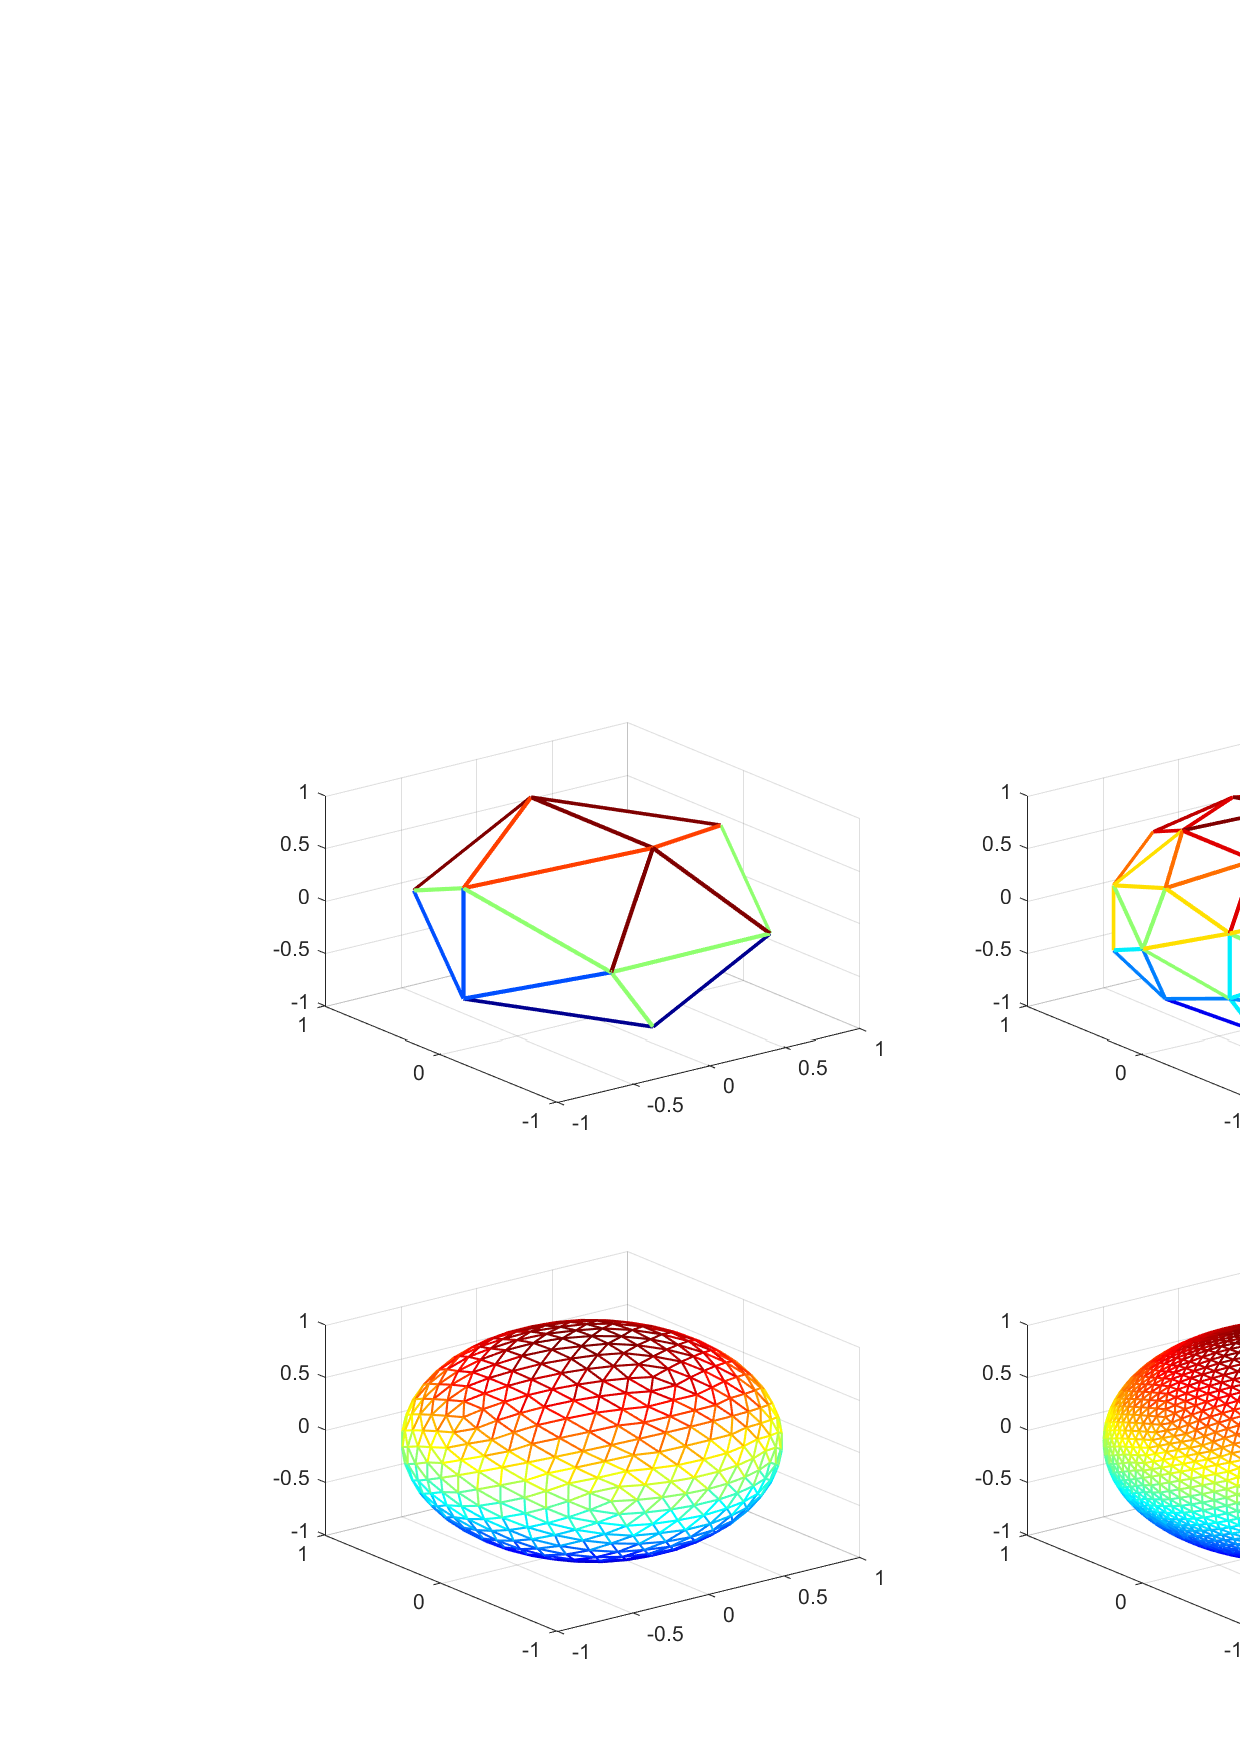
\includegraphics[scale = 0.5]{./figs/facet.png} \: 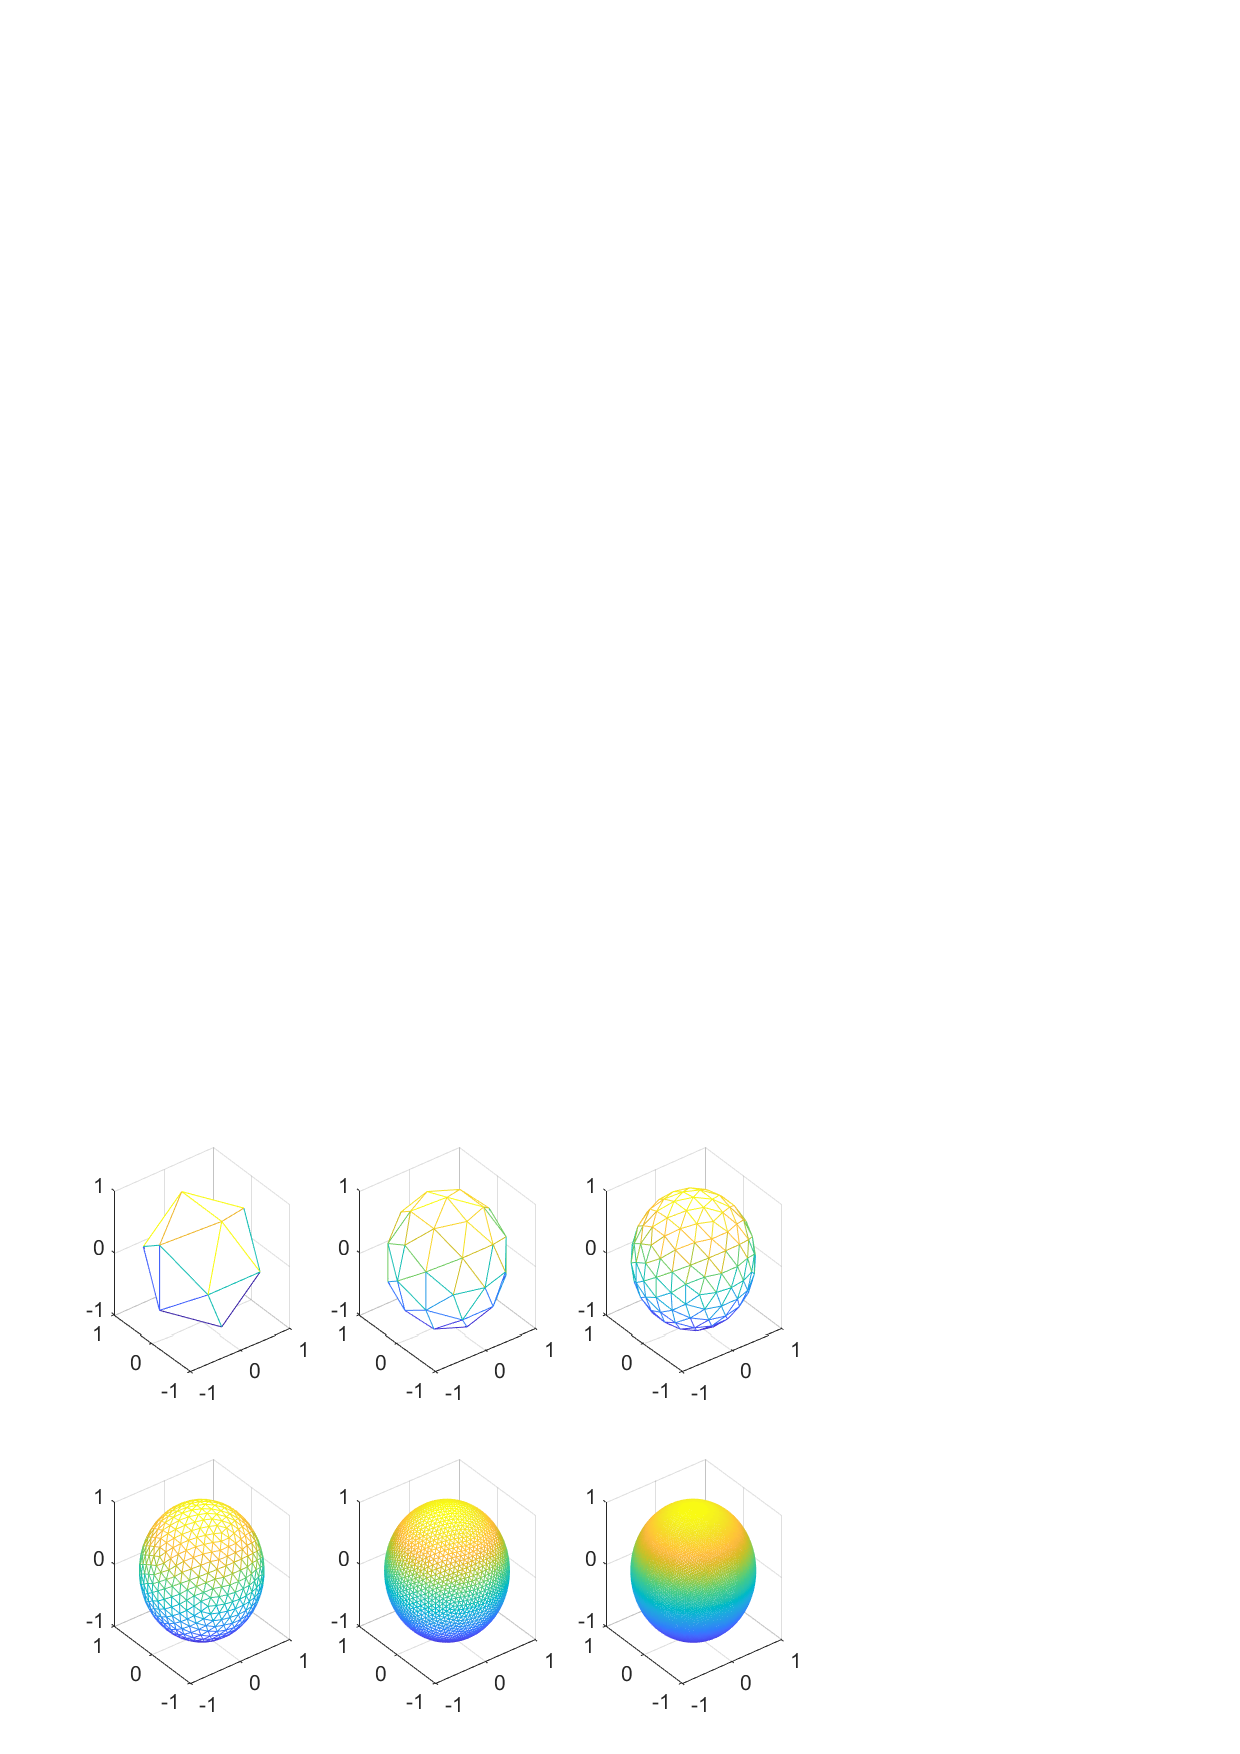
\includegraphics[scale = 0.5]{./figs/icosahedron.png}}
\end{frame}



\begin{frame}[t]
\frametitle{Conclusion and future work}
\begin{itemize}
\item Implicit representations of composite objects readily obtained from R-functions 
\item Advantages of continuous OCS computation over facet method for simple shapes
\item 
\item Investigation of continuous solutions for more complex/``sharper" objects 
\end{itemize}
\end{frame}

\end{document}
